\documentclass[conference]{IEEEtran}
\usepackage{todonotes}
%\todo{Make a cake}
\usepackage{url}
\usepackage{lipsum}
% Basically, \url{my_url_here}.

% *** CITATION PACKAGES ***
%
\usepackage{cite}
% \cite{} output to follow that of the IEEE.
% The documentation is contained in the cite.sty file itself.

% *** MATH PACKAGES ***
%
%\usepackage{amsmath}
% A popular package from the American Mathematical Society that provides
% many useful and powerful commands for dealing with mathematics.
%
% Note that the amsmath package sets \interdisplaylinepenalty to 10000
% thus preventing page breaks from occurring within multiline equations. Use:
%\interdisplaylinepenalty=2500
% after loading amsmath to restore such page breaks as IEEEtran.cls normally
% does. amsmath.sty is already installed on most LaTeX systems. The latest
% version and documentation can be obtained at:
% http://www.ctan.org/pkg/amsmath

% *** ALIGNMENT PACKAGES ***
\usepackage{array}
\usepackage{tikz,tabularx,amsthm,amsmath,amssymb,amsfonts,listings,xcolor,enumerate,url,array,
	multirow,forest}

% *** SUBFIGURE PACKAGES ***
%\ifCLASSOPTIONcompsoc
%  \usepackage[caption=false,font=normalsize,labelfont=sf,textfont=sf]{subfig}
%\else
%  \usepackage[caption=false,font=footnotesize]{subfig}
%\fi
% subfig.sty, written by Steven Douglas Cochran, is the modern replacement
% for subfigure.sty, the latter of which is no longer maintained and is
% incompatible with some LaTeX packages including fixltx2e. However,
% subfig.sty requires and automatically loads Axel Sommerfeldt's caption.sty
% which will override IEEEtran.cls' handling of captions and this will result
% in non-IEEE style figure/table captions. To prevent this problem, be sure
% and invoke subfig.sty's "caption=false" package option (available since
% subfig.sty version 1.3, 2005/06/28) as this is will preserve IEEEtran.cls
% handling of captions.
% Note that the Computer Society format requires a larger sans serif font
% than the serif footnote size font used in traditional IEEE formatting
% and thus the need to invoke different subfig.sty package options depending
% on whether compsoc mode has been enabled.
%
% The latest version and documentation of subfig.sty can be obtained at:
% http://www.ctan.org/pkg/subfig


% *** Do not adjust lengths that control margins, column widths, etc. ***
% *** Do not use packages that alter fonts (such as pslatex).         ***
% There should be no need to do such things with IEEEtran.cls V1.6 and later.
% (Unless specifically asked to do so by the journal or conference you plan
% to submit to, of course. )


% correct bad hyphenation here
\hyphenation{op-tical net-works semi-conduc-tor}


\begin{document}
%
% paper title
% Titles are generally capitalized except for words such as a, an, and, as,
% at, but, by, for, in, nor, of, on, or, the, to and up, which are usually
% not capitalized unless they are the first or last word of the title.
% Linebreaks \\ can be used within to get better formatting as desired.
% Do not put math or special symbols in the title.
\title{Title of the article}


% author names and affiliations
% use a multiple column layout for up to three different
% affiliations
\author{\IEEEauthorblockN{Mahieddine Yaker\\ and Julien Cartigny \\and Gilles Grimaud}
\IEEEauthorblockA{IRCICA\\
University of Lille\\
address in Lille\\
Email: yyy@yyy.com}
\and
\IEEEauthorblockN{Chrystel Gaber \\ and Xiao Han \\ and Vicente Sanchez-Leighton}
\IEEEauthorblockA{Orange Labs,\\
Ch\^{a}tillon, France\\
Email: firstname.lastname@orange.com\\}
}

% conference papers do not typically use \thanks and this command
% is locked out in conference mode. If really needed, such as for
% the acknowledgment of grants, issue a \IEEEoverridecommandlockouts
% after \documentclass

% for over three affiliations, or if they all won't fit within the width
% of the page, use this alternative format:
% 
%\author{\IEEEauthorblockN{Michael Shell\IEEEauthorrefmark{1},
%Homer Simpson\IEEEauthorrefmark{2},
%James Kirk\IEEEauthorrefmark{3}, 
%Montgomery Scott\IEEEauthorrefmark{3} and
%Eldon Tyrell\IEEEauthorrefmark{4}}
%\IEEEauthorblockA{\IEEEauthorrefmark{1}School of Electrical and Computer Engineering\\
%Georgia Institute of Technology,
%Atlanta, Georgia 30332--0250\\ Email: see http://www.michaelshell.org/contact.html}
%\IEEEauthorblockA{\IEEEauthorrefmark{2}Twentieth Century Fox, Springfield, USA\\
%Email: homer@thesimpsons.com}
%\IEEEauthorblockA{\IEEEauthorrefmark{3}Starfleet Academy, San Francisco, California 96678-2391\\
%Telephone: (800) 555--1212, Fax: (888) 555--1212}
%\IEEEauthorblockA{\IEEEauthorrefmark{4}Tyrell Inc., 123 Replicant Street, Los Angeles, California 90210--4321}}

% make the title area
\maketitle

% As a general rule, do not put math, special symbols or citations
% in the abstract
\begin{abstract}
Abstract \todo[inline]{TBD}
%%\lipsum[1]
\end{abstract}

% no keywords




% For peer review papers, you can put extra information on the cover
% page as needed:
% \ifCLASSOPTIONpeerreview
% \begin{center} \bfseries EDICS Category: 3-BBND \end{center}
% \fi
%
% For peerreview papers, this IEEEtran command inserts a page break and
% creates the second title. It will be ignored for other modes.
\IEEEpeerreviewmaketitle



\section{Introduction}
\label{sec:Intro}
% no \IEEEPARstart
\todo[inline]{TBD}
%\lipsum[1-2]
\hfill mds
 
\hfill March 05, 2018


\section{Internet of Things security issues}

Oravec and co \cite{Oravec2017} described in their paper the increase of utilization of devices and applications dedicated to Internet of Things, particularly in the case of household appliances and house management. They wished to demonstrated the new issues that should be considered with the expansion of IoT into the house. One of their main concern is the security and privacy integrity. They descried some scenario about attack or other information leak due to fallible devices. In the case before us, Sivaraman and co\cite{Sivaraman2016}, described a scenario based on an attack of all house IoT devices via a smartphone application. After scanning all available devices in the house with the smartphone, they show how they can get control of each IoT device into the house. With this attack, they show that even if there is strong network security mechanisms, if any component of the House IoT has any application level "problem", the security and privacy is no more guaranteed into the house. This attack works with a smartphone, but we can also imagine a scenario where an another connected to internet device (Webcam, connected TV..) can be a perfect attack vector. 





\section{Isolation model}
\label{sec:Isolation_model}
\todo[inline]{TBD by Lille}
%\lipsum[1-10]
\subsection{Memory isolation proto-kernel}

\begin{figure}
	\centering
	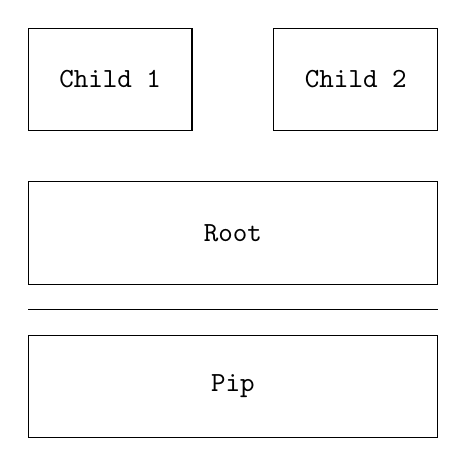
\begin{tikzpicture}[baseline=0, scale=2.6]
	% Draw rectangles
	\draw(-1, -2) rectangle (1, -1.5);
	\draw(-1, -1.25) rectangle (1, -0.75);
	\draw(-1, -0.5) rectangle (-0.2, 0);
	\draw(0.2, -0.5) rectangle (1, 0);
	
	% Draw kernel-user separation
	\draw[-] (-1,-1.375) -- (1, -1.375);
	
	% Draw text
	\draw (0,-1.75) node{\texttt{Pip}} ;
	\draw (0,-1) node{\texttt{Root}} ;
	\draw (-0.6,-0.25) node{\texttt{Child 1}} ;
	\draw (0.6,-0.25) node{\texttt{Child 2}} ;
	\end{tikzpicture}
	\caption{Pip architecture view} 
	\label{fig:PipArchBase}
\end{figure}



PIP\cite{bergougnoux2017} is a protokernel: it allows for kernels, ranging from hypervisors to monolithic kernels, to be developed as user mode applications (figure \ref{fig:PipArchBase}). This means that only PIP is executed in kernel mode (i.e., the privileged mode of the hardware)(figure . Indeed, code running in kernel mode has direct access to the whole memory and hardware. It is thus clearly better, from a security point of view, to keep this code as minimal as possible. This stems from the general principle that the trusted computing base (TCB) should be kept minimal. One of the PIP key design is to have a minimal number of functionalities while ensuring strong isolation. More precisely, PIP only manages memory isolation and redirection of interruptions to user space code, and has only 10 system calls. Contrary to micro-kernel, it means that components like scheduler, IPC and authorization are not included in the PIP kernel, neither other mechanism available in monolithic kernel like device abstraction layer, file systems, network stack, etc.



\begin{figure}[h!]
	%	\begin{minipage}[c]{5.1cm}
	%	\end{minipage}
	\hfill
	%	\begin{minipage}[c]{0.65\linewidth}
	
	\centering
	\begin{forest}
		for tree={grow=east,reversed,minimum height=0.7cm}
		[P$_{\mbox{root}}$
		[P$_1$
		[P$_{1.1}$
		[P$_{1.1.1}$]
		[P$_{1.1.2}$]
		[P$_{1.1.3}$]
		]
		[P$_{1.2}$
		[P$_{1.2.1}$]
		[P$_{1.2.2}$]
		]
		]
		[P$_2$
		[P$_{2.1}$]
		[P$_{2.2}$]
		]
		]
	\end{forest}
	\caption{The view by Pip of the partition tree}
	\label{abstree:fig}
	%	\end{minipage}
\end{figure}
PIP proposes a hierarchic  memory isolation model (figure \ref{abstree:fig}) to partition the available memory among several memory-limited space called partition. A partition is a set of physical memory pages mapped to virtual address. At start, all the available memory (as defined inside PIP configuration) makes up the ROOT partition. The root partition can include mapped registers from hardware devices, thus providing access to hardware functionalities. Code executed in a parent partition can request (via system calls to PIP) segregation to its memory space: a new child partition is created on which the parent partition can mapped a subset of its own mapped physical memory pages, thus \textit{delegating} part of its memory space to the child partition. This model is recursive: any partition can create a child partition and delegate part of its memory space. While a partition can read and write in the memory of its child partition (we call this property vertical sharing), sibling partitions cannot access each other's memory (we call this property horizontal isolation).
\subsection{Pip API}
In order to deal with partitions mechanisms, Pip provides a set of function for creation and deletion.

\subsection{Interrupt management}
To manage interruptions, PIP has two different behaviours depending of the kind of interruption:
\begin{itemize}
	\item Software interrupts (fault or system calls) are relayed to the parent partition (with the exception of the PIP system calls).
	\item Hardware interrupts are relayed to the ROOT partition which is in charge to forward it to, for instance, a network card driver.
\end{itemize}

The hierarchic isolation model approach offers a hierarchic \textbf{security} model: a child parent partition can only access physical memory pages delegated by its parent. Furthermore, a parent receives all software interruptions from its children%\footnote{With the notable exception of the PIP system calls, as a partition can create sub-partitions only based on a (sub)set of its own memory space, thus not breaking the hierarchic isolation model.}
, thus controlling which interactions have its children with the system.

\subsection{Message passing}
Due to Pip isolation mechanism, the only way for a partition to communicate with others is to use Pip interrupt mechanism. Pip provide to partitions a function called \textit{dispatch()} which permit to send a signal with datas to its parent or one of its child partition. This function is a call to Pip API, and after some verification, Pip send the signal to destination. This Pip call is the only requirement to implement an IPC between partitions.



\section{Industrial ecosystem}
\label{sec:Industrial_ecosystem}
This section aims at describing the industrial ecosystem and the needs for a security architecture based on isolation. First, we identify and define the stakeholders involved in the use and management of an IOT or M2M device. The responsibilities of each actor are then described and finally, the requirements for an isolation-based architecture are listed.\\

In this section, we consider that a domain is an isolated area which belongs to an entity. The notion of domain is further precised in section \ref{sec:Domain_def}.\\

We distinguish device ressources and domain ressources. Device ressources correspond to the isolated partitions (domains) and the ressources exposed by software installed in the manufacturer or owner domains or the sensors \& actuators drivers. Domain ressources correspond to the ressources that are exposed by a particular domain and created by applications or services in this domain.\\

\subsection{Actors}
\label{sec:Actors}
We identify 6 stakeholders, namely the manufacturer, maintainer, owner, administrator, service provider and user, which interact with the IOT ot M2M device.
\subsubsection{Manufacturer}
It issues the device and the isolation solution. It also provides each device an identifier that will subsequently allow it to be identified as well as intial secrets that will allow the owner to access the device. It may also provide the drivers and software components for the sensors or actuators on the device. 
\subsubsection{Maintainer}
It maintains the device, monitors the hardware components status and applies the patches deliveres by the manufacturer. This role can either be assumed or delegated to a third party by the manufacturer. 
\subsubsection{Owner}
The device belongs to the Owner who defines an access policy to authorize which other entities are authorized to use or manage the device or domains within the device. The Owner can possess several devices. It receives initial credentials from the manufacturer that allows it to access each device in his fleet. 
\subsubsection{Administrator}
It enforces the policy defined by the owner for his fleet of devices. If any modification, such as adding a new entity or modifying its granted permissions,  is required, it requests a decision from the owner. This role can either be assumed or delegated to a third party by the owner. 
\subsubsection{Service Provider}
It delivers a user-friendly service on one or multiple devices using the ressources authorized by the Owner. It installs or activates a service within the device. Muliple Service Providers can co-exist on the same device. 
\subsubsection{User}
Users consume the services provided by the entities mentioned above. We can distinguish platform users and technical users. Service users subscribe to the services provided by the Service Providers. Technical users are typically members of the Owner, Manufacturer, Maintainer entities and they will perform authorized administration actions such as creating a new domain, granting rights to a new user, loading a service on the device. In the rest of this article we focus on platform users. 
\subsection{Responsibilities model}
\label{sec:Resp_model}

The manufacturer provides the mechanisms and temporary credentials to personalize the device. At delivery, it provides the keys of the owner domain. The manufacturer is responsible for providing drivers which are compatible with virtualization and usage by multiple entities. For example, to control the position of an armed robot, it is better to literally express the coordinates of the destination. The command "go to (x=10;y=40;z=20)" leads to less confusion than "go to current position + (x=10; y=20; z=30). The manufacturer provides a platform in a safe state to the owner and does not keep any access to the manufacturer domain. In particular, the manufacturer does not manage access control to the drivers.\\

The Owner finalizes the personalization of the device after delivery by the manufacturer. In particular, the owner should modify its temporary credentials. Owner authorizes the usage of the device resources. If some resources are very sensitive, he provides the access to them through the use of a token which he delivers and verifies. The owner can choose that some resources are accessible freely without the use of a token and thus reducing the security. The owner must not have any control or visibility on the actions performed by other entities unless it touches sensitive functions which the owner has decided to control through token verification.\\

If the owner delegates his tasks to an administrator, then the administrator can configure which resources need to be accessed with a token and the administrator is responsible for verifying the token and should not be able to control or visualize the actions performed by other actors unless they concern his perimeter of action.\\

The maintainer keeps the firmware, driver or any software in his perimeter up to date. This responsibility is key in the future as the regulators start to take actions on this point. For instance, the European Commission's overall security strategy \cite{enisa_iot_2017} requires vendors to the commit to update their software in the event of newly disclosed vulnerabilities, as part of "duty of care" principle. Such initiative also exists in the United States with the Internet Of Things (IoT) Cybersecurity Improvement Act of 2017 \cite{IOTAct_2017}.\\

Any entity which owns a partition (administrator, service provider, and maintainer) has to authenticate the machine (or user) who is sending the commands to the partition. This entity can choose to not perform and access control verification, thus reducing the security of the system. Any entity which owns a partition (administrator, service provider, and maintainer) is responsible for modifying the temporary credentials of its associated domains.\\

The responsibilities described in this section are summarized in table \ref{tab:resp_table}.\\

\begin{table*}[!ht]
% increase table row spacing, adjust to taste
\renewcommand{\arraystretch}{1.3}
% if using array.sty, it might be a good idea to tweak the value of
% \extrarowheight as needed to properly center the text within the cells
\caption{Responsibilities matrix}
\label{tab:resp_table}
\centering
% Some packages, such as MDW tools, offer better commands for making tables
% than the plain LaTeX2e tabular which is used here.
\begin{tabular}{|p{8cm}||c|c|c|c|c|c|}
\hline
Requirements & Manufacturer & Maintainer & Owner & Administrator & Service Provider\\
\hline
Provide mechanisms \& temporary credentials for initial device personalization before delivery to the owner & X & & & &\\
\hline
Provide drivers compatible with virtualization \& multi-tenant usage & X & & & &\\
\hline
Provide temporary credentials for initial domain personalization to entities after delivery to the owner & & & X & X & \\
\hline
Update regularly the credentials to access the domain under its responsibility & X & X & X & X & X\\
\hline
Provide the device to owner without a remote backdoor access & X & & & & \\
\hline
Create / Modify / Delete a domain before delivery to owner & X & & & & \\
\hline
Create / Modify / Delete a domain after delivery to owner & & & X & X & \\
\hline
Configure the access policy of the device ressources & & & X & & \\
\hline
Enforce the device ressource access policy & & & X & X & \\
\hline
Configure the domain ressource access policy & X & X & X & X & X \\
\hline
Enforce the domain ressource access policy & X & X & X & X & X \\
\hline
Keep the firmware \& drivers up to date & X & X & & & \\
\hline
Keep the service applications up to date & & & & & X \\
\hline
\end{tabular}
\end{table*}

\subsection{Architecture requirements}
\label{sec:Arch_req}

\subsubsection{Domain isolation}
Two services which run in two isolated domains should not be able to access the memory of one another, gain information about each other or interfere with each other's execution. 

\subsubsection{Owner non-interference}
Although the owner or the administrator have access to a privileged domain, they must not have any control or visibility on the actions performed by other entities if these actions do not involve device ressources which are under the responsibility of the owner.

\subsubsection{Ressource access control}
A device ressource access policy under the control of the owner or the administrator is mandatory. For each domain, a domain ressource access policy under the control of the domain owner (maintainer, service provider) is optional. 

\subsubsection{Minimal on-device processing}
The processing required to authorize an action in the device must be minimal. 

\section{Proposed Security model and architecture}
\label{sec:Architecture}
This section describes the architecture based on the use of tokens proposed in the ODSI project. First, we define the notion of domain in this architecture as well as its components. Then, we describe the communication and management models.
\subsection{Definition of a domain}
\label{sec:Domain_def}
In this architecture, the device is shared between several parties with different roles (described in section \ref{sec:Actors}). As one party can execute various code in different space, the following vocabulary is used:
\begin{itemize}
    \item A partition is a piece of code managed by one party with its own memory
    \item A domain is the union of all partitions managed by one party.
\end{itemize}
\todo[inline]{Do we design ODSI platform \& ODSI Mesovisor specifically in this article ?}
Domains are implemented in ODSI Mesovisor via the hierarchical memory model. As the memory space of partition can contain the (disjoint) memory space of several sub-partitions (which can themselves contains others sub-sub-partitions), the parent partition controller by one party is the party domain and every enclosed partitions are controlled by the same party.


\subsection{Components of a domain}
\label{sec:Domain_comp}
This section describes the role of the components which enforce the proposed security model, namely the Configuration Manager, the Administration Manager, the Token \& Security Validator and the Key Vault. The architecture is also based on the use of virtual sensors and actuators. 

\subsubsection{Configuration Manager}
\label{sec:Config_Mgr}
The Configuration Manager can be divided into two functions and sub-components, the isolation manager and the internal communication manager. The isolation manager provides the tools to create, read, modify or delete a domain. This module also contains a security policy which indicates which tasks and partitions should be started when the domain is started. This security policy also creates the communication channels between the tasks and partitions in the domain. The internal communication manager is the unique entry point of the domain. 

\subsubsection{Virtual sensors or actuators}
\label{sec:virtual_sensor}
The drivers are provided by the manufacturer of the device and are stored in a separate domain. Each domain contains a virtual sensor or actuator which exposes the functions of the actual sensor or actuator and acts as an interface with it. This allows the entity which owns the domain to see his domain as an actual device without knowledge of the isolation. The instruction and response are transmitted to and from the real driver using the internal communication mechanism.  

\subsubsection{Administration Manager}
\label{sec:Admin_Mgr}
This module exposes the domain's ressources to an external server managed by the entity which owns the domain. It routes the command to read, write, execute the ressource to the expected manager or virtual sensor, actuator. It sends each command received to the Token \& Security Validator (T\&S Validator). 

\subsubsection{Token \& Security Validator}
\label{sec:Token_Validator}
The Token \& Security Validator (T\&S Validator) validates each device management command against the token provided in the command and optionnally an internal security policy. For example, the security policy defines which ressources require a token verification to be accessed or whether a specific command can be processed accordaccording to the device battery status. 

\subsubsection{Key Vault}
\label{sec:Key_Vault}
This module stores the keys that are used by the domain. In particular, the keys used by the Token \& Security Valdiator are stored here. It also provides the functions to add a new key, modify or delete an existing key.

\subsection{Management model}
\label{sec:Management_model}
\todo[inline]{Image ?}
The model proposed is based on a master/agent model. Each domain contains an agent, the administration manager which receives commands from a master, generally an application in a server.
\subsubsection{Token scheme}
The token format should contain at minimum a payload and a signature of this payload. Compatible token formats include JWT (JSON Web Token) \cite{rfc7519_jwt_2015} and CWT (CBOR Web Token) \cite{rfc_CWT_2017}.\\

The token's objectives are to 1) ensure that any command will reach the intended destination, 2) give the rights to request some operations on ressources, 3) prove that the entity initiating the command has been authenticated authorized and protect against replay.

In order to achieve these goals, the token should contain at minimum:
\begin{itemize}
    \item the ID of the partition to which this token is destined,
    \item the rights granted,
    \item a proof ensuring that the token was generated by the token provider,
    \item a token ID and/or an expiration date.
\end{itemize}

The proof can either be a digital signature, such as ANS X9.31, ANS X9.62 or PKCS\#1 as recommended by NIST \cite{nist_dss_2013} or a Keyed-hash Message Authentication Codes (HMACS) compliant NIST recommendations and using a NIST-approved hash algorithm such as SHA-256 \cite{nist_hmac_2008, nist_hash_2012}, depending on the level of security and non-repudiation required.
The token ID and expiration date are used to prevent replay. The token ID can be compared to a set of previously used IDs stored in a cache. The size of the cache should be adapted to the memory constraints of the partition and device. The combination of the size of the cache and the expiration date allows achieving best effort replay detection. Therefore, it is strongly recommended to use both elements and to tune them carefully. 

\subsubsection{Domain ressources management}
%\lipsum[1-6]
\subsubsection{Device ressources management}
%\lipsum[1-6]

\subsection{Communication model}
\label{sec:Communication_model}
\todo[inline]{TBD. Section to be described by Lille}
The main requirement for the communication protocol is to allow master/agent communication and the transport of a payload with the command content and an associated token. Protocols such as TCP/IP or CoAP are eligible. LwM2M \cite{oma_lwm2M_2017} cannot be used as such because it does not allow adding the token in its payload.

\subsubsection{Internal communication}
%\lipsum[1-6]
\subsubsection{External communication}
%\lipsum[1-6]


\section{Evaluation}
\todo[inline]{TBD. Section to show how the isolation model allows to address the industrial needs}

For the scenario described above\cite{Sivaraman2016}, we can use our proposed security architecture and Pip to avoid this kind attack on any household devices. 

The memory isolation provided by Pip avoid any memory leak or other attacks based on memory issues or hardware access. The only way for any Partition to have an interaction with others, is to use the communication mechanism provided by Pip. If any malicious partition wants to threaten an other one, the only attack vector available is through the communication mechanism, a partition can . However, with the token mechanism provided by the ODSI architecture, there is only authorized command that can be send to others partitions. That's why, the attacker has less possibilities to take access or execute unwanted commands into others partitions.



%\lipsum[1-4]

\section{Conclusion}
\todo[inline]{TBD. The conclusion goes here. Next steps : implementation and performance evaluation}
%\lipsum[1-2]



% conference papers do not normally have an appendix


% use section* for acknowledgment
\section*{Acknowledgment}
This article was done in the scope of the European Celtic-Plus project ODSI.  





% trigger a \newpage just before the given reference
% number - used to balance the columns on the last page
% adjust value as needed - may need to be readjusted if
% the document is modified later
%\IEEEtriggeratref{8}
% The "triggered" command can be changed if desired:
%\IEEEtriggercmd{\enlargethispage{-5in}}

% references section

% can use a bibliography generated by BibTeX as a .bbl file
% BibTeX documentation can be easily obtained at:
% http://mirror.ctan.org/biblio/bibtex/contrib/doc/
% The IEEEtran BibTeX style support page is at:
% http://www.michaelshell.org/tex/ieeetran/bibtex/
%\bibliographystyle{IEEEtran}
% argument is your BibTeX string definitions and bibliography database(s)
%\bibliography{IEEEabrv,../bib/paper}
%
% <OR> manually copy in the resultant .bbl file
% set second argument of \begin to the number of references
% (used to reserve space for the reference number labels box)

% An example of a floating figure using the graphicx package.
% Note that \label must occur AFTER (or within) \caption.
% For figures, \caption should occur after the \includegraphics.
% Note that IEEEtran v1.7 and later has special internal code that
% is designed to preserve the operation of \label within \caption
% even when the captionsoff option is in effect. However, because
% of issues like this, it may be the safest practice to put all your
% \label just after \caption rather than within \caption{}.
%
% Reminder: the "draftcls" or "draftclsnofoot", not "draft", class
% option should be used if it is desired that the figures are to be
% displayed while in draft mode.
%
%\begin{figure}[!t]
%\centering
%\includegraphics[width=2.5in]{myfigure}
% where an .eps filename suffix will be assumed under latex, 
% and a .pdf suffix will be assumed for pdflatex; or what has been declared
% via \DeclareGraphicsExtensions.
%\caption{Simulation results for the network.}
%\label{fig_sim}
%\end{figure}

% Note that the IEEE typically puts floats only at the top, even when this
% results in a large percentage of a column being occupied by floats.


% An example of a double column floating figure using two subfigures.
% (The subfig.sty package must be loaded for this to work.)
% The subfigure \label commands are set within each subfloat command,
% and the \label for the overall figure must come after \caption.
% \hfil is used as a separator to get equal spacing.
% Watch out that the combined width of all the subfigures on a 
% line do not exceed the text width or a line break will occur.
%
%\begin{figure*}[!t]
%\centering
%\subfloat[Case I]{\includegraphics[width=2.5in]{box}%
%\label{fig_first_case}}
%\hfil
%\subfloat[Case II]{\includegraphics[width=2.5in]{box}%
%\label{fig_second_case}}
%\caption{Simulation results for the network.}
%\label{fig_sim}
%\end{figure*}
%
% Note that often IEEE papers with subfigures do not employ subfigure
% captions (using the optional argument to \subfloat[]), but instead will
% reference/describe all of them (a), (b), etc., within the main caption.
% Be aware that for subfig.sty to generate the (a), (b), etc., subfigure
% labels, the optional argument to \subfloat must be present. If a
% subcaption is not desired, just leave its contents blank,
% e.g., \subfloat[].

\bibliographystyle{unsrt}
\bibliography{biblio}





% that's all folks
\end{document}


